\documentclass{beamer}
\usepackage{xltxtra}
\defaultfontfeatures{Ligatures=TeX}
\usepackage[american]{babel}
\usepackage{setspace}
\usepackage{color}
\usepackage{hyperref}
\hypersetup{
  colorlinks=true,
  linkbordercolor = {white},
}
\usepackage{listings}

\mode<presentation>

\begin{document}
\title{MediaTek LinkIt\texttrademark\ Smart 7688 Duo Development Platform}
\author[freedom]{Koan-S\^in T\^an \\ \href{mailto:freedom@acm.org}{freedom@acm.org}}

\begin{frame}
  \titlepage
\end{frame}

\begin{frame}
  \frametitle{What is it?}
  \begin{itemize}
  \item an affordable development board (7688: \$12.9, 7688 Duo: \$15.90)
    \begin{itemize}
    \item Linklt Smart 7688: MPU only. Powered by MediaTek MIPS-based Wi-Fi AP SoC \href{http://labs.mediatek.com/fileMedia/download/9ef51e98-49b1-489a-b27e-391bac9f7bf3}{MT7688AN}.
    \item Linklt Smart 7688 Duo: MPU and MCU. Powered by MediaTek MT7688 and \href{http://www.atmel.com/devices/atmega32u4.aspx}{ATmega32U4}.
    \end{itemize}
  \item key features:
    \begin{itemize}
    \item 580 MHz MIPS CPU
    \item Single input single output(1T1R) Wi-Fi 802.11 b/g/n (2.4 GHz)
    \item Pin-out for GPIO, I2C, SPI,UART, PWM, and Ethernet port
    \item 32MB Flash and 128MB DDR2 RAM
    \item USB host
    \item Micro SD slot
    \item Support for Arduino (ATmega32U4)
    \end{itemize}
  \item OS: \href{https://openwrt.org/}{OpenWrt} 15.05
  \item Programming environment: C/C++ (cross-compiling), Python, and Node.js
    \begin{itemize}
    \item well, it's Linux. You can put whatever you like into your microSDHC and microSDXC cards
    \end{itemize}
  \end{itemize}
\end{frame}

\begin{frame}
\end{frame}

\begin{frame}[fragile]
  \begin{lstlisting}
    make[1] world
    make[2] target/compile
    make[3] -C target/linux compile
    make[2] package/cleanup
    make[2] package/compile
    make[3] -C package/libs/toolchain compile
    make[3] -C package/libs/libnl-tiny compile
    make[3] -C package/libs/libjson-c compile
    make[3] -C package/utils/lua compile
    make[3] -C package/libs/libubox compile
    make[3] -C package/system/ubus compile
    make[3] -C package/system/uci compile
    make[3] -C package/network/config/netifd compile
    make[3] -C package/system/opkg host-compile
    make[3] -C package/system/ubox compile
    make[3] -C package/libs/lzo compile
    make[3] -C package/libs/zlib compile
    make[3] -C package/libs/ncurses host-compile
  \end{lstlisting}
\end{frame}

\begin{frame}[fragile]
  \begin{lstlisting}
    make[3] -C package/libs/ncurses compile
    make[3] -C package/utils/util-linux compile
    make[3] -C package/utils/ubi-utils compile
    make[3] -C package/system/procd compile
    make[3] -C package/system/usign host-compile
    make[3] -C package/utils/jsonfilter compile
    make[3] -C package/system/usign compile
    make[3] -C package/base-files compile
    make[3] -C package/system/fstools compile
    make[3] -C package/boot/uboot-envtools compile
    make[3] -C package/libs/libreadline compile
    make[3] -C package/devel/gdb compile
    make[3] -C package/devel/strace compile
    make[3] -C feeds/linkit/mtk-linkit-webui compile
    make[3] -C package/network/utils/wireless-tools compile
    make[3] -C feeds/linkit/mtk-sdk-wifi compile
    make[3] -C feeds/luci/modules/luci-base host-compile
    make[3] -C package/libs/libtool compile
  \end{lstlisting}
\end{frame}

\begin{frame}[fragile]
  \begin{lstlisting}
    make[3] -C feeds/packages/libs/libjpeg compile
    make[3] -C feeds/packages/multimedia/mjpg-streamer compile
    make[3] -C package/utils/lua host-compile
    make[3] -C feeds/luci/applications/luci-app-mjpg-streamer compile
    make[3] -C package/network/services/samba36 compile
    make[3] -C feeds/luci/applications/luci-app-samba compile
    make[3] -C feeds/luci/libs/luci-lib-json compile
    make[3] -C feeds/luci/themes/luci-theme-openwrt compile
    make[3] -C package/firmware/linux-firmware compile
    make[3] -C package/kernel/linux compile
    make[3] -C package/network/utils/iptables compile
    make[3] -C package/network/config/firewall compile
    make[3] -C feeds/luci/applications/luci-app-firewall compile
    make[3] -C feeds/luci/libs/luci-lib-ip compile
    make[3] -C feeds/luci/libs/luci-lib-nixio compile
    make[3] -C package/network/utils/iwinfo compile
    make[3] -C package/system/rpcd compile
    make[3] -C feeds/luci/modules/luci-base compile
  \end{lstlisting}
\end{frame}

\begin{frame}[fragile]
  \begin{lstlisting}
    make[3] -C feeds/luci/modules/luci-mod-admin-full compile
    make[3] -C feeds/luci/protocols/luci-proto-ppp compile
    make[3] -C feeds/luci/themes/luci-theme-bootstrap compile
    make[3] -C package/libs/polarssl compile
    make[3] -C package/libs/ustream-ssl compile
    make[3] -C package/network/services/uhttpd compile
    make[3] -C feeds/luci/protocols/luci-proto-ipv6 compile
    make[3] -C feeds/luci/collections/luci compile
    make[3] -C feeds/packages/libs/alsa-lib compile
    make[3] -C feeds/packages/utils/alsa-utils compile
    make[3] -C feeds/packages/libs/expat compile
    make[3] -C feeds/packages/utils/dbus compile
    make[3] -C feeds/packages/libs/gdbm compile
    make[3] -C feeds/packages/libs/intltool host-compile
    make[3] -C feeds/packages/libs/libdaemon compile
    make[3] -C feeds/packages/libs/avahi compile
    make[3] -C feeds/packages/libs/avahi compile
    make[3] -C feeds/packages/libs/confuse compile
  \end{lstlisting}
\end{frame}

\begin{frame}[fragile]
  \begin{lstlisting}
    make[3] -C package/libs/libusb compile
    make[3] -C feeds/packages/libs/libftdi1 compile
    make[3] -C package/utils/bzip2 compile
    make[3] -C package/libs/gettext compile
    make[3] -C package/libs/libiconv compile
    make[3] -C package/libs/argp-standalone compile
    make[3] -C package/libs/elfutils compile
    make[3] -C package/libs/libusb-compat compile
    make[3] -C feeds/packages/utils/avrdude compile
    make[3] -C feeds/packages/net/cgi-io compile
    make[3] -C feeds/packages/utils/attr compile
    make[3] -C feeds/packages/utils/acl compile
    make[3] -C package/libs/gmp compile
    make[3] -C feeds/packages/utils/coreutils compile
    make[3] -C feeds/packages/kernel/exfat-nofuse compile
    make[3] -C package/libs/ocf-crypto-headers compile
    make[3] -C package/libs/openssl compile
    make[3] -C package/network/utils/curl compile
  \end{lstlisting}
\end{frame}

\begin{frame}[fragile]
  \begin{lstlisting}
    make[3] -C package/system/ca-certificates compile
    make[3] -C feeds/packages/net/git compile
    make[3] -C feeds/packages/libs/hidapi compile
    make[3] -C feeds/packages/libs/libuv compile
    make[3] -C feeds/packages/libs/expat host-compile
    make[3] -C package/utils/bzip2 host-compile
    make[3] -C feeds/packages/lang/python host-compile
    make[3] -C feeds/packages/lang/node compile
    make[3] -C feeds/packages/lang/node host-compile
    make[3] -C feeds/packages/libs/libxml2 compile
    make[3] -C package/libs/uclibc++ compile
    make[3] -C feeds/packages/libs/db47 compile
    make[3] -C feeds/packages/libs/libffi compile
    make[3] -C feeds/packages/libs/sqlite3 compile
    make[3] -C feeds/packages/lang/python compile
    make[3] -C feeds/packages/utils/swig host-compile
    make[3] -C feeds/packages/libs/libmraa compile
    make[3] -C feeds/packages/libs/libupm compile
  \end{lstlisting}
\end{frame}

\begin{frame}[fragile]
  \begin{lstlisting}
    make[3] -C feeds/packages/libs/libid3tag compile
    make[3] -C feeds/packages/libs/libmad compile
    make[3] -C feeds/packages/sound/madplay compile
    make[3] -C feeds/packages/lang/node-serialport compile
    make[3] -C feeds/packages/lang/node-arduino-firmata compile
    make[3] -C feeds/packages/lang/node-cylon compile
    make[3] -C feeds/packages/lang/node-hid compile
    make[3] -C feeds/packages/lang/python-setuptools compile
    make[3] -C feeds/packages/lang/python-pip compile
    make[3] -C feeds/packages/lang/python-pyserial compile
    make[3] -C feeds/packages/utils/spi-tools compile
    make[3] -C feeds/packages/utils/yunbridge compile
    make[3] -C package/system/mountd compile
    make[3] -C feeds/linkit/mtk-linkit compile
    make[3] -C package/kernel/gpio-button-hotplug compile
    make[3] -C package/network/config/swconfig compile
    make[3] -C package/network/ipv6/odhcp6c compile
    make[3] -C package/network/services/dnsmasq compile
  \end{lstlisting}
\end{frame}

\begin{frame}[fragile]
  \begin{lstlisting}
    make[3] -C package/network/services/dropbear compile
    make[3] -C package/network/services/hostapd compile
    make[3] -C package/network/services/odhcpd compile
    make[3] -C package/libs/libpcap compile
    make[3] -C package/network/utils/linux-atm compile
    make[3] -C package/network/utils/resolveip compile
    make[3] -C package/network/services/ppp compile
    make[3] -C package/system/mtd compile
    make[3] -C package/system/opkg compile
    make[3] -C package/utils/busybox compile
    make[2] package/install
    make[3] package/preconfig
    make[2] target/install
    make[3] -C target/linux install
    make[2] package/index
  \end{lstlisting}
\end{frame}

\begin{frame}
  \frametitle{Some Caveats}
  \begin{itemize}
  \item if you don't like FAT, vFAT, and exFAT, build your own kernel
  \item `make menuconfig' or `make kernel\_menuconfig' in OpenWrt building environment
  \item zeroconf and dual-stack problem: use http://ipv4-address or http://ipv6-address instead of http://something.local
  \item surely it's easier to use USB flash drive to update firmware
  \item NOT all the packages in OpenWrt are tested to be built on OS X
  \begin{itemize}
  \item adding /opt/local/libexec/gnubin to PATH helps a lot
  \item /bin/tar
  \item gyp, node\_gyp
  \end{itemize}
  \end{itemize}
\end{frame}

\begin{frame}
  \begin{itemize}
  \item bootloader, u-boot, \href{https://github.com/MediaTek-Labs/linkit-smart-7688-uboot}{source code}
  \item kernel, 3.18-based, \href{http://git.openwrt.org/15.05/openwrt.git?p=15.05/openwrt.git;a=tree;f=target/linux/ramips/patches-3.18;hb=HEAD}{here}
    \begin{itemize}
    \item some of them are upstreamed to mainline, some are not (yet)
    \item one big exception now is the Wi-Fi driver
    \item should be possible to use mainline kernel
    \end{itemize}
  \item Since there is lua, we can build lua-rs232 and use it to communicate with Arduino
  \end{itemize}
\end{frame}

\begin{frame}
  \begin{figure}
    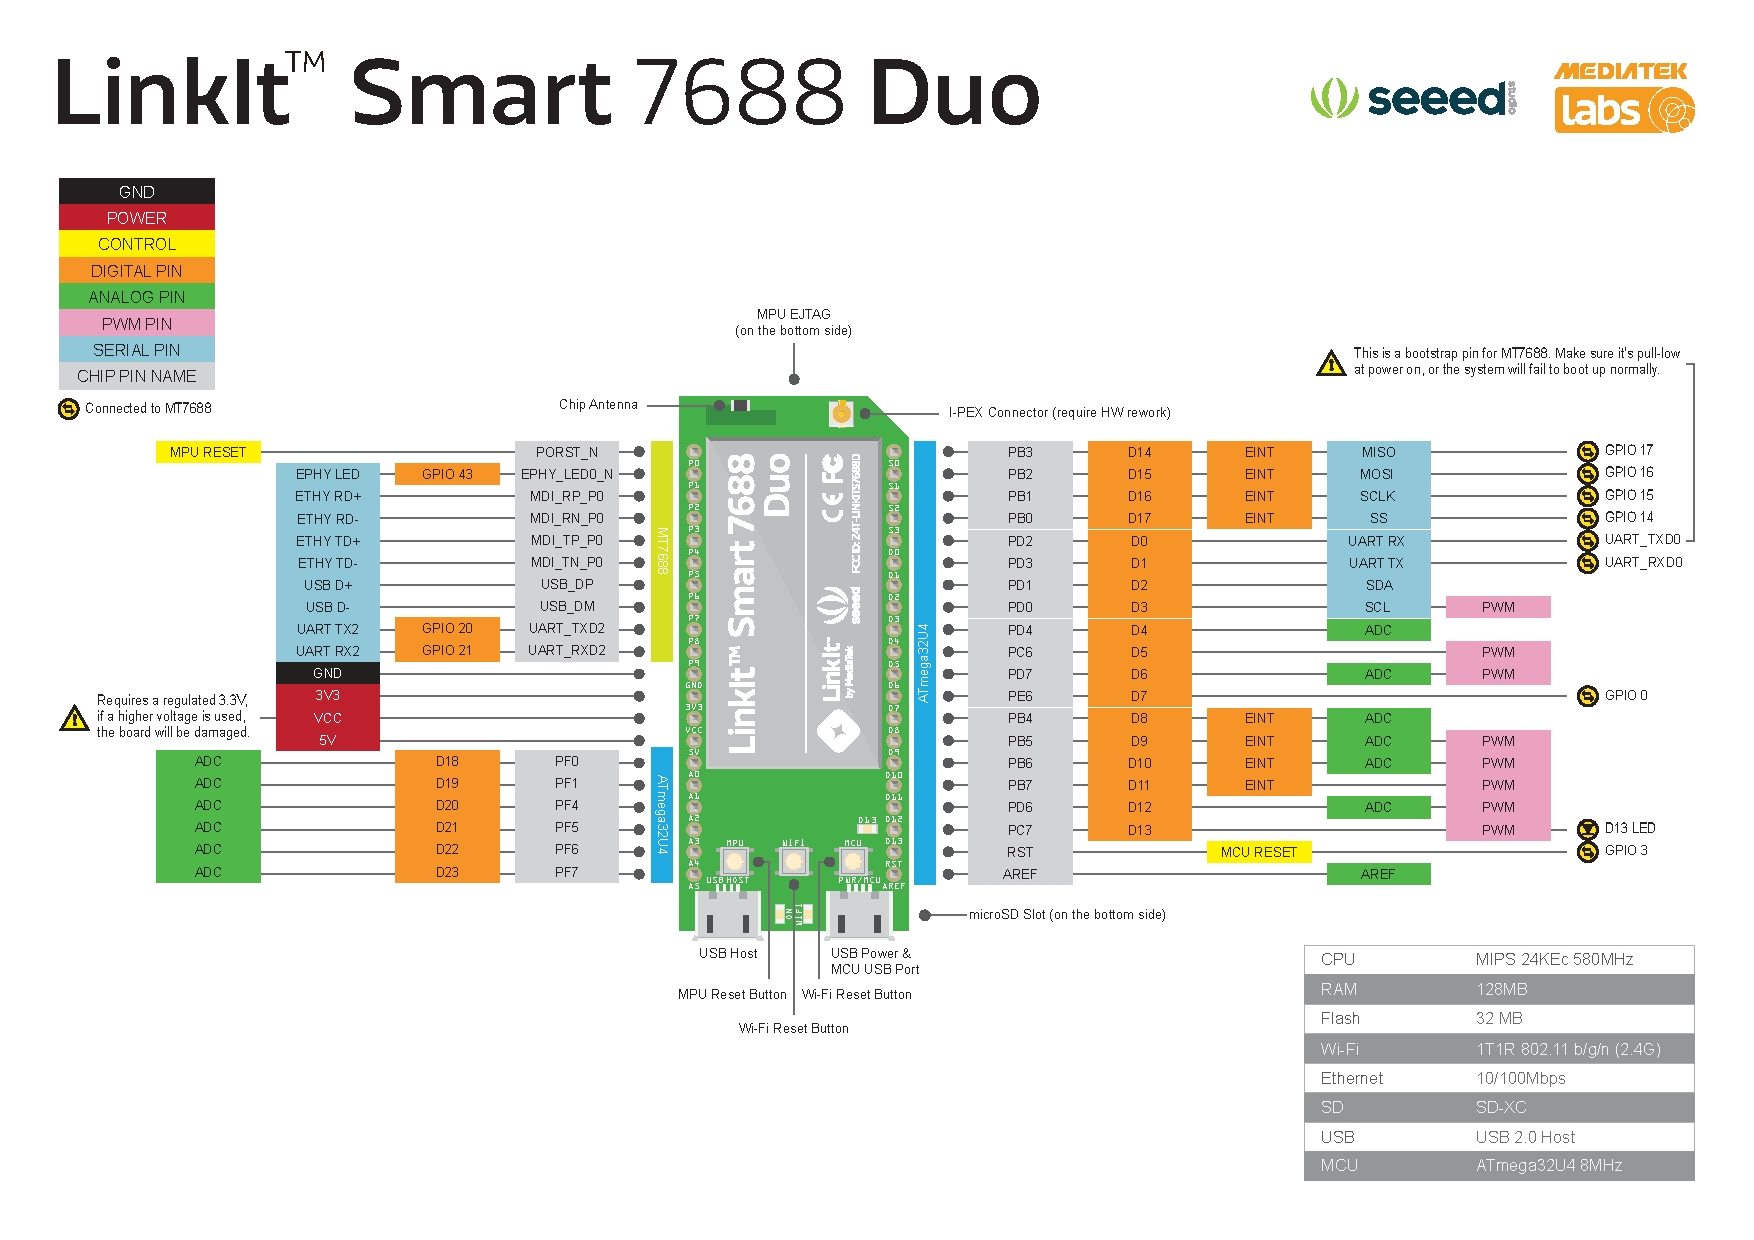
\includegraphics[height=\textheight,width=\textwidth,keepaspectratio]{pin.pdf}
  \end{figure}
\end{frame}

\begin{frame}
  \begin{figure}
    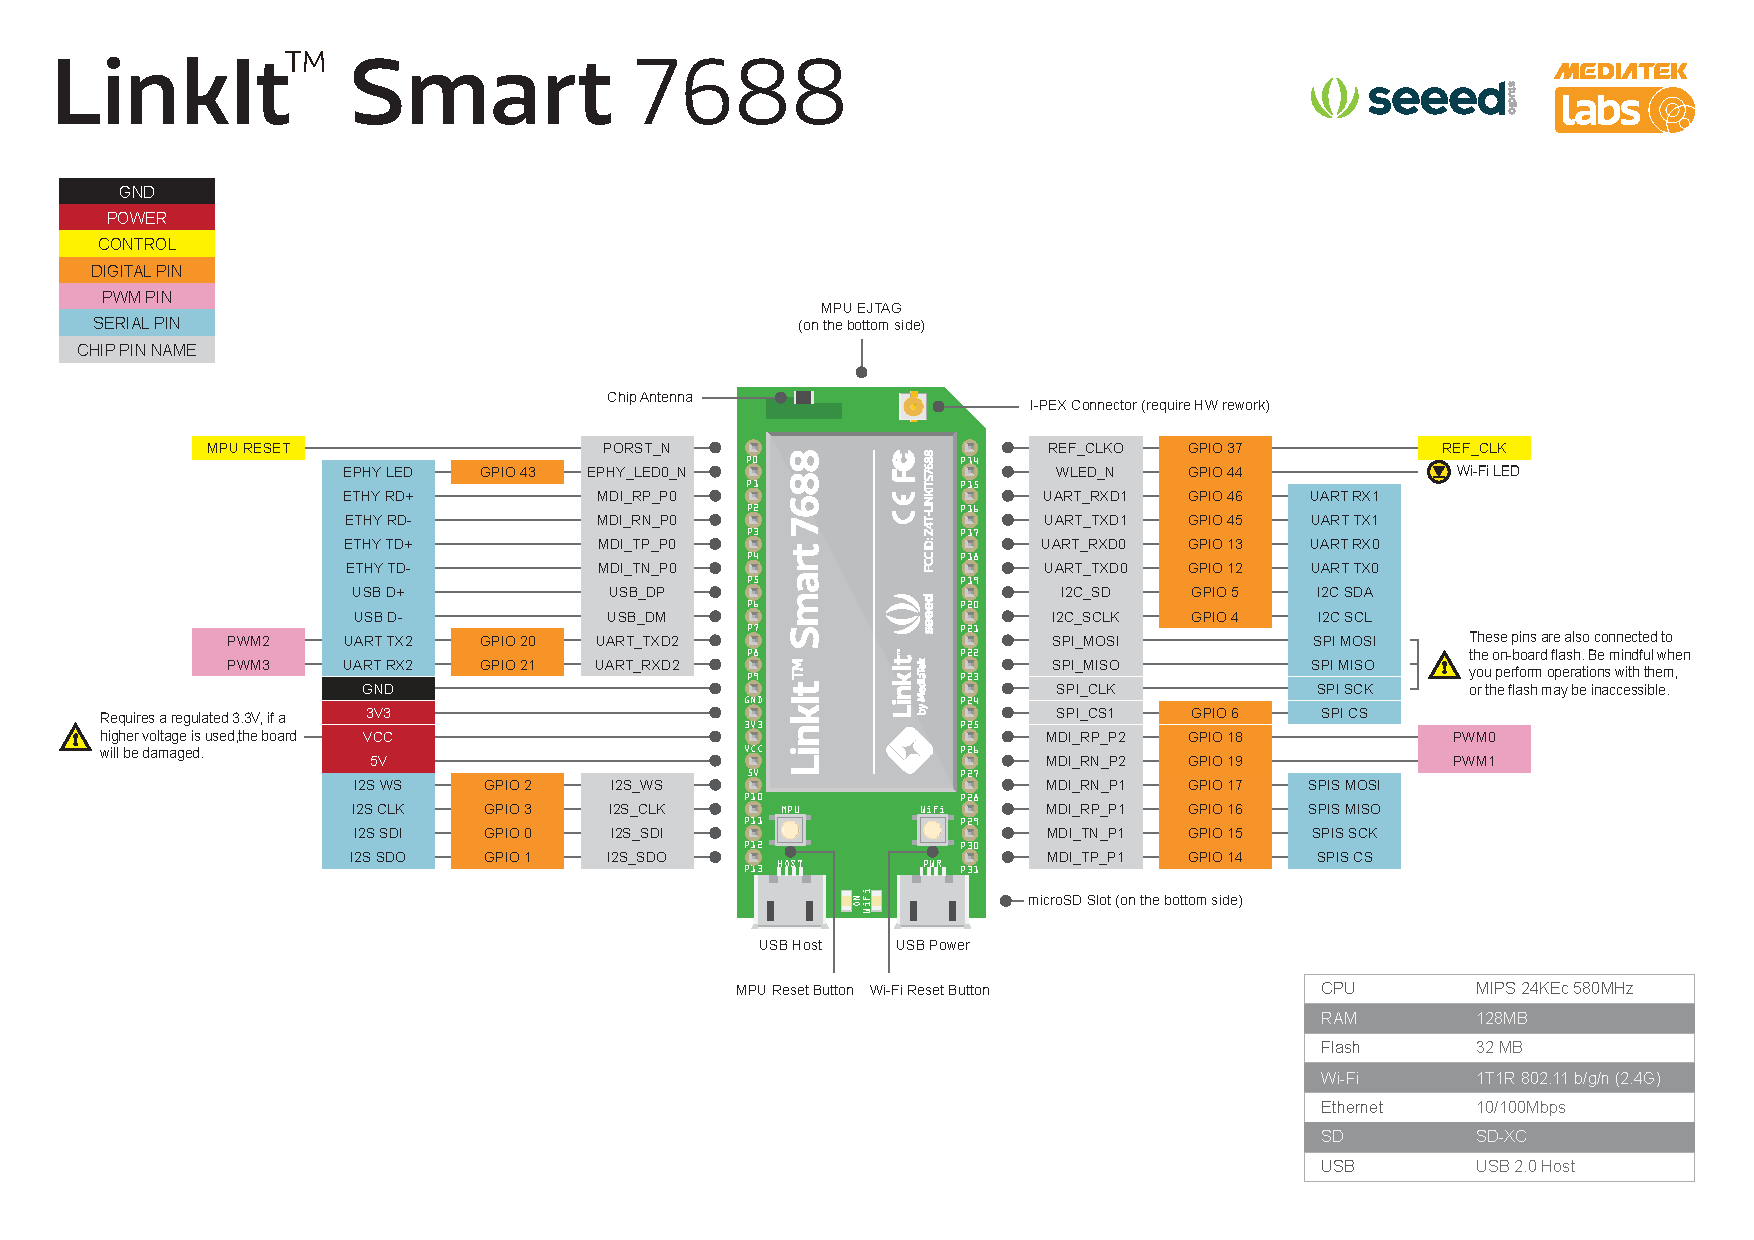
\includegraphics[height=\textheight,width=\textwidth,keepaspectratio]{pin2.pdf}
  \end{figure}
\end{frame}

\end{document}
